% 2011 年辽宁卷文科第 21 题：椭圆 C1、C2 与直线 l。
% 来源 PDF：普通高考/2011/2011辽宁文.pdf，SHA-256 29407891a0a44aaa00db6398312f058fc98c005913323db3729a50333cec4564。
% 原页：第 2 页第 2 栏中部，书页码 684。示意。
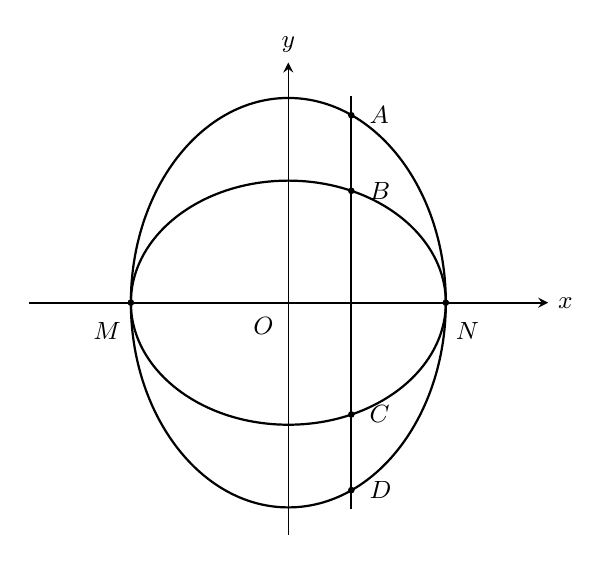
\begin{tikzpicture}[>=stealth, semithick, font=\small, scale=1.0]
  \draw[->] (-3.3,0)--(3.3,0) node[right] {$x$};
  \draw[->] (0,-2.95)--(0,3.05) node[above] {$y$};
  \draw[thick] (0,0) ellipse (2 and 1.55);
  \draw[thick] (0,0) ellipse (2 and 2.6);
  \draw[thick] (0.8,-2.62)--(0.8,2.62);
  \fill (0.8,2.38) circle (1.2pt) node[right=3pt] {$A$};
  \fill (0.8,1.42) circle (1.2pt) node[right=3pt] {$B$};
  \fill (0.8,-1.42) circle (1.2pt) node[right=3pt] {$C$};
  \fill (0.8,-2.38) circle (1.2pt) node[right=3pt] {$D$};
  \fill (-2,0) circle (1.2pt);
  \fill (2,0) circle (1.2pt);
  \node[below left] at (-2,-0.12) {$M$};
  \node[below right] at (2,-0.12) {$N$};
  \node[below left] at (-0.06,-0.06) {$O$};
\end{tikzpicture}
